% !TeX root = ../thuthesis-example.tex

\chapter{研究背景}
\label{background}
在机器人学研究中,视觉惯性测距(VIO)在导航、定位和感知任务中发挥着举足轻重的作用。VIO 系统通过融合来自视觉和惯性传感器的数据来估计机器人的姿态(位置和方向)。近年来,人们提出了许多 VIO 方法,例如直接使用像素强度估算摄像机运动的直接方法,以及基于特征的方法等。其中,基于特征的方法使用图像特征(点、线或平面)来估计传感器位姿和周围环境的地图。
\begin{figure}
  \centering
  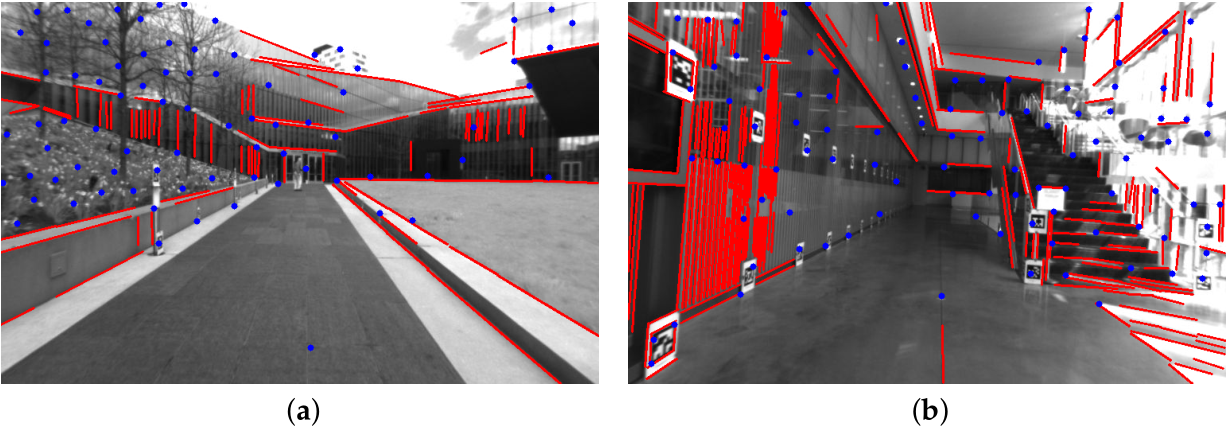
\includegraphics[width = 0.75\textwidth]{plbg.png}
  \label{fig_plbg}
  \caption{图像中的点线特征}
\end{figure}
基于点的 VIO 算法发展最为成熟,现有点VIO算法在精度和速度方面都表现出了卓越的性能,可以应用于需要实时跟踪的场景。然而,在低纹理环境或重复纹理环境中(例如走廊、道路、开阔水域等),由于点特征信息匮乏,基于点的 VIO 算法会出现性能下降的问题。为了利用环境中丰富的边缘信息,克服点信息失效的问题,研究人员进一步开发了基于线特征的VIO算法,并将线特征作为辅助构建了点线联合的VIO框架,现有框架包括PL-SLAM[4],PL-VINS[5]等。但是,由于线特征存在参数化复杂且耗时的问题,现有的点线联合VIO框架难以在嵌入式设备上实时运行,使得线特征的精度增益难以在小型无人设备(比如无人机)上得到实现。 为了构建一个可以在嵌入式小型无人设备上实时运行的点线VIO系统,本工作首先基于神经网络的特征推理网络,提出了点线融合的SP-SOLD2网络,并利用自监督训练使得该网络可以通过一次推理得到特征点、特征线以及同时适用于点线匹配的描述子;为了将各类点线提取和匹配方法灵活应用于VIO任务中,本工作构建了一个前端方法可自定义的NN-PL-VIO框架,并利用SP-SOLD2点线联合网络以及一系列速度优化方法,得到了一个可以在嵌入式设备Orin NX上实时运行的点线联合VIO系统。

\section{点特征提取及描述方法}
点特征提取方法可以简单地分类为传统方法和深度学习方法两大类,其中传统方法是通过一系列数学计算得到特征点及其描述子,具有数学可解释性;而深度学习方法则是通过设计网络来端到端推理定位特征点,和描述子可以不耦合。一些常见的传统点特征方法如下:
\begin{enumerate}
  \item Harris角点检测算法(Harris Corner Detection):该算法通过计算图像中每个像素点的角点响应函数来检测角点。角点响应函数基于图像中局部区域的亮度变化,对角点位置具有较高的响应值。Harris角点检测算法具有旋转不变性和一定程度的尺度不变性。
  \item Shi-Tomasi角点检测算法(Shi-Tomasi Corner Detection):该算法是对Harris角点检测算法的改进。它使用了一个更加鲁棒的角点响应函数,能够在保持高角点检测率的同时提供更好的角点定位精度。
  \item SIFT(尺度不变特征变换,Scale-Invariant Feature Transform):SIFT是一种广泛应用的特征点提取算法,能够在不同尺度和旋转条件下提取稳定的特征点。SIFT算法通过在图像中检测局部极值点,并在多个尺度上计算尺度空间特征向量,得到具有尺度不变性的特征描述子。
  \item SURF(加速稳健特征,Speeded-Up Robust Features):SURF算法是对SIFT算法的改进,通过提出一种快速的特征点检测和描述子计算方法,实现了更高的计算效率。SURF算法利用图像的Hessian矩阵来检测特征点,并使用Haar小波响应描述子来描述特征。
  \item FAST(Features from Accelerated Segment Test):FAST算法是一种快速的角点检测算法,适用于实时应用。该算法基于像素灰度值的变化来检测角点,通过高效的特征点筛选策略提高了检测速度。
  \item ORB(Oriented FAST and Rotated BRIEF):ORB算法是对FAST和BRIEF(Binary Robust Independent Elementary Features)算法的结合。它在FAST算法的基础上引入了旋转不变性,并使用二进制描述子来进行特征匹配,具有较高的计算效率和良好的性能。
\end{enumerate}
而基于神经网络的点特征提取方法可以分为两种类别:检测和描述分离的方法与端到端匹配的方法。其中检测和描述分离的方法是设计两个网络或者一个联合网络,分别进行点特征的检测和点描述子的提取;而端到端匹配的方法则是直接设计和训练一个网络,此网络可以接受两个输入图像,直接给出特征匹配结果。基于神经网络的方法总结如下表:
\begin{table}[!ht]
  \centering
  \begin{tabular}{|c|c|c|}
  \hline
      名称 & 类型 & 描述 \\ \hline
      ASLFeat[6] & 点检测 & \parbox[c]{6cm}{使用可变形卷积网络,利用固有的特征层次,提出了一种多级检测机制,该机制不仅在没有额外学习权重的情况下可以恢复低层细节以进行精确的关键点定位} \\ \hline
      SuperPoint[7] & 点检测和描述子提取联合 & \parbox[c][15ex]{6cm}{介绍了一个自监督框架,利用运行在全尺寸图像上的全卷积模型,在一个前向传递中同时计算像素级兴趣点位置和关联描述子} \\ \hline
      R2D2[8] & 点检测和描述子提取联合 & \parbox[c]{6cm}{在D2-Net基础上考虑了特征检测的可重复性和可靠性,为检测得分设计了损失函数,使用全卷积网络推理特征点及其描述子} \\ \hline
      LoFTR[9] & 端到端匹配 &\parbox[c]{6cm}{ 使用了Transformer中的自我和交叉注意力层(self and cross attention layers)来获取两个图像的特征描述符,实现无检测器的局部特征匹配。} \\ \hline
      Patch2Pix[10] & 端到端匹配 & \parbox[c]{6cm}{建立了一种新的匹配细化网络,首先得到 patch-level 的匹配,再细化到 pixel-level 的匹配,网络可以同时细化匹配并排除错误匹配,且训练不需要像素级的 GT 对应关系。} \\ \hline
      SuperGlue[11] & 描述子提取 & \parbox[c]{6cm}{提出了一种能够同时进行特征匹配以及滤除外点的网络,基于注意力机制提出了一种灵活的内容聚合机制,这其能够同时感知潜在的3D场景以及进行特征匹配。} \\ \hline
  \end{tabular}
\end{table}

\section{研究背景}
test

\section{各章节概述}
\label{outline}
本研究报告共分为六章,本章主要介绍了本研究的背景、现存挑战,从应用和学术研究的角度阐述了本研究的必要性和挑战性。第二章至第四章分别介绍了仿真器的改进工作、强化学习算法和部署平台的结构设计,并简要介绍这些设计对总体飞行性能的影响。第五章介绍了本研究的实验结果,包括仿真平台参数的设置,算法调试的结果和实机部署的结果。第六章对本研究做一个整体总结并提出该项目未来可继续改进的方向。


% \section{引言的写法}

% 一篇学位论文的引言大致包含如下几个部分:
% 1、问题的提出;
% 2、选题背 景及意义;
% 3、文献综述;
% 4、研究方法;
% 5、论文结构安排。
% \begin{itemize}
%   \item 问题的提出:要清晰地阐述所要研究的问题“是什么”。
%     \footnote{选题时切记要有“问题意识”,不要选不是问题的问题来研究。}
%   \item 选题背景及意义:论述清楚为什么选择这个题目来研究,即阐述该研究对学科发展的贡献、对国计民生的理论与现实意义等。
%   \item 文献综述:对本研究主题范围内的文献进行详尽的综合述评,“述”的同时一定要有“评”,指出现有研究状态,仍存在哪些尚待解决的问题,讲出自己的研究有哪些探索性内容。
%   \item 研究方法:讲清论文所使用的学术研究方法。
%   \item 论文结构安排:介绍本论文的写作结构安排。
% \end{itemize}



% \section{正文的写法}

% 本部分是论文作者的研究内容,不能将他人研究成果不加区分地掺和进来。
% 已经在引言的文献综述部分讲过的内容,这里不需要再重复。
% 各章之间要存在有机联系,符合逻辑顺序。



% \section{结论的写法}

% 结论是对论文主要研究结果、论点的提炼与概括,应精炼、准确、完整,使读者看后能全面了解论文的意义、目的和工作内容。
% 结论是最终的、总体的结论,不是正文各章小结的简单重复。
% 结论应包括论文的核心观点,主要阐述作者的创造性工作及所取得的研究成果在本领域中的地位、作用和意义,交代研究工作的局限,提出未来工作的意见或建议。
% 同时,要严格区分自己取得的成果与指导教师及他人的学术成果。

% 在评价自己的研究工作成果时,要实事求是,除非有足够的证据表明自己的研究是“首次”、“领先”、“填补空白”的,否则应避免使用这些或类似词语。
